% ---* APENDICE *---
% Escribir el algoritmo original y el modificado

\chapter{Experimento: Agrupando Métodos de Test}\aplabel{exp-clustering}

\par Un problema del \emph{approach} de \emph{TestSurgeon} es la gran cantidad  comparaciones 1-a-1 entre tests, en el caso de {\tt ROMondrianViewBuilderTest} al contener 96 tests, se deben realizar potencialmente $\frac{1}{2} \cdot 96 \cdot (96-1) = 4.560$ comparaciones. Muchas de estas son innecesarias debido a que los tests se enfocan en partes del sistema muy distintas o sin ninguna relación. Una manera de reducir estas comparaciones es agrupar tests similares y así realizar comparaciones entre elementos de estos grupos solamente. La característica de los tests a comparar es su cobertura, ya que entre mayor sea ésta, más chances de encontrar un caso de refactorización/restructuración. 

\par Para esto se decidió utilizar el algoritmo de \textbf{Agrupación Aglomerativo Jerárquico} (o \textbf{Hierarchical Agglomerative Clustering }, \textbf{HAC}). El cual en cada paso fusionar los dos clusters más cercanos, partiendo con $N$ clusters que contienen 1 solo elemento y hacer esto hasta que quede 1 cluster con $N$ elementos formando una jerarquía. Entonces, al terminar su ejecución, el usuario puede solicitar la partición con $k$ clusters. 

\par Sin embargo no se sabe cuántos clusters se necesitan. Pero sí se sabe que los clusters deben tener una similitud interna suficiente para que las comparaciones sean fructíferas y no una pérdida de tiempo. La experiencia indica que para que esto suceda la similitud entre un par de tests debe ser de al menos un 80\%, por lo cual la similitud interna de cada cluster (promedio entre las similitudes de todos los pares de tests en el cluster) debe ser al menos de un 75\%. 

\par Por otro lado, tampoco se sabe qué medida de distancia entre clusters es la más apropiada para este problema: \emph{Single Link}, \emph{Complete Link} o \emph{Average Link} \footnote{La definición formal de cada una de la métricas se presenta en la \secref{impl-hac}}.  

\section{Metodología}

\par Entonces, para determinar los mejores parámetros para correr el algoritmo HAC se realizó un experimento en el cual se ejecutó el algoritmo variando tanto la distancia utilizada como la similitud interna mínima exigida. Las tolerancias de similitud interna ($s_{min}$) variaron de la siguiente forma: 95\%, 90\%, 85\%, 80\% y 75\%.

\par Para la evaluación se consideraron las siguientes condiciones de una ``buena agrupación'':
\begin{description}
\item[Condición \#1] El cluster no-unitario con menor $s$ deben tener buena similitud interna (ojalá varios puntos porcentuales más que $s_{min}$).
\item[Condición \#2] Los clusters no-unitarios no deben ser tan distintos en su tamaño. Es decir se debe evitar que haya un cluster gigante y muchos pequeños que es justamente el problema inicial.
\item[Condición \#3] Debe tener pocos clusters unitarios. Y los que existan deben ser suficientemente distintos a los demás clusters.
\end{description}

\par El otro criterio complementario a los anteriores es el número total de comparaciones con la nueva agrupación de test. Esta métrica asume que no se harán comparaciones de elementos entre clusters. Para el caso de $k$ clusters donde $\texttt{size}(C_i)$ corresponde al número de elementos que contiene el $i$-ésimo cluster , el total de comparaciones se calcula como:


   \[ \sum_{i=1}^{k} \frac{1}{2} \,\, \texttt{size(}C_i\texttt{)} \times \left( \texttt{size(}C_i\texttt{)} -1 \right) \]


\section{Resultados}

% Interpretar los resultados, eleccion de la mejor. 
\par Como resultado de este experimento se obtuvo 15 configuraciones representadas en pares (\emph{distancia} , $s$). Cada una de estas están graficadas en forma de anillo en la \figref{ap-clustering}, clasificadas verticalmente según la distancia utilizada y horizontalmente según el valor de $s_{min}$. Como era de esperar, a mayor $s_{min}$ se obtuvieron mayor cantidad de clusters independientemente de la distancia escogida, y a medida que la $s_{min}$ disminuía una cantidad menor de clusters pero más heterogéneos. En la gráfica de anillo, cada punto (o vértice del polígono) representa un cluster, y su distancia del centro del anillo representa su valor de similitud interna. Así los puntos que están en el borde externo del anillo corresponden a clusters con $s=100\%$ y que generalmente corresponden a clusters que nunca se fusionaron y contienen un solo elemento, a los cuales informalmente les llamaremos \textit{unitarios}.


%================ FIGURA DE CLUSTERING
%\cleardoublepage % que este en una pagina nueva
\begin{figure}
\centering
\setlength{\tabcolsep}{1pt} % reducir la separacion entre columnas
\begin{tabular}[t]{cccc}
& \textbf{Single Link} & \textbf{Complete Link} & \textbf{Average Link} \\
% \textbf{95\%}
\subfloat{
\includegraphics[height=3.9cm]{images/clustering/95.pdf}}
   & \subfloat[45 Clusters]{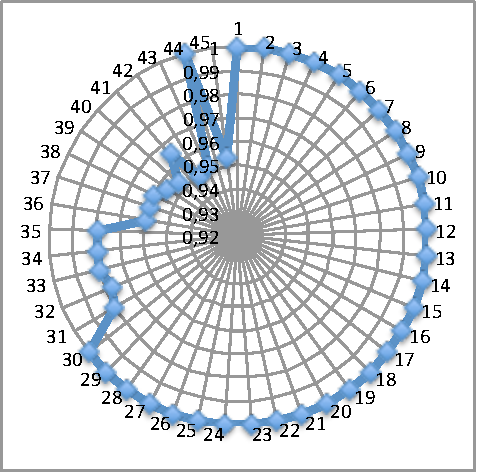
\includegraphics[width=3.9cm]{images/clustering/sl-95.pdf}} 
   & \subfloat[51 Clusters]{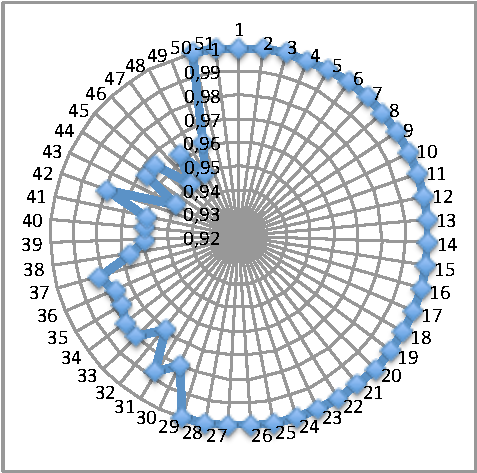
\includegraphics[width=3.9cm]{images/clustering/cl-95.pdf}}
   & \subfloat[47 Clusters]{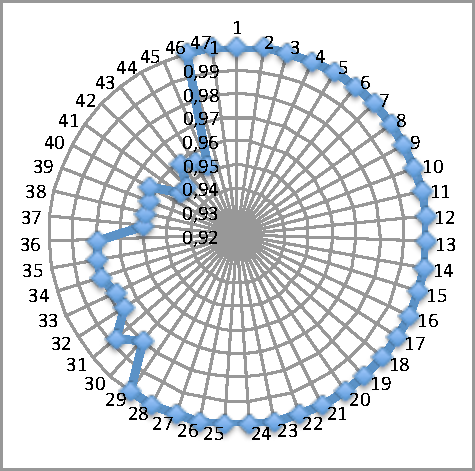
\includegraphics[width=3.9cm]{images/clustering/al-95.pdf}} \\[-0.1in] % reducir la separacion entre filas 

% \textbf{90\%}
\subfloat{
\includegraphics[height=3.9cm]{images/clustering/90.pdf}}
   & \subfloat[27 Clusters]{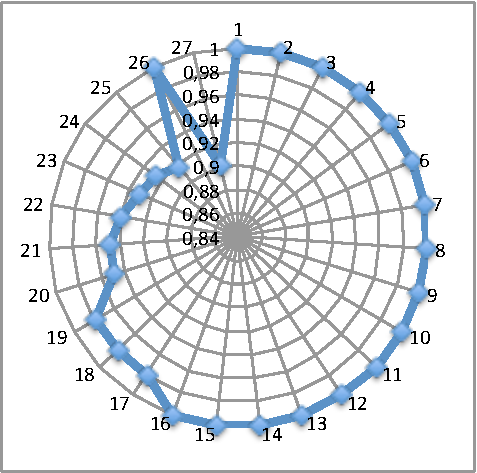
\includegraphics[width=3.9cm]{images/clustering/sl-90.pdf}} 
   & \subfloat[37 Clusters]{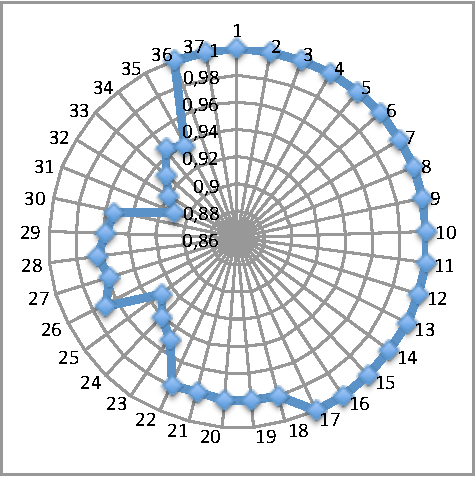
\includegraphics[width=3.9cm]{images/clustering/cl-90.pdf}}
   & \subfloat[29 Clusters]{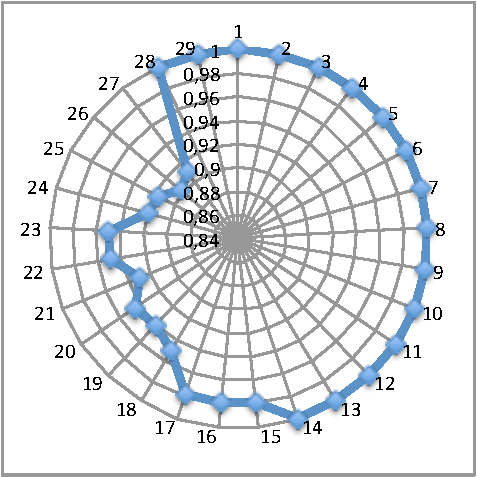
\includegraphics[width=3.9cm]{images/clustering/al-90.pdf}} \\[-0.1in]

% \textbf{85\%}
\subfloat{
\includegraphics[height=3.9cm]{images/clustering/85.pdf}}
   & \subfloat[22 Clusters]{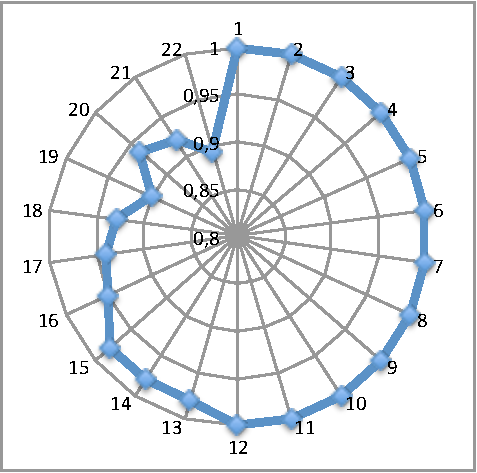
\includegraphics[width=3.9cm]{images/clustering/sl-85.pdf}} 
   & \subfloat[22 Clusters]{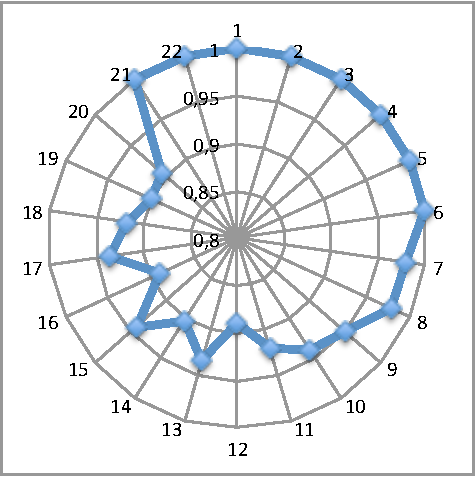
\includegraphics[width=3.9cm]{images/clustering/cl-85.pdf}}
   & \subfloat[20 Clusters]{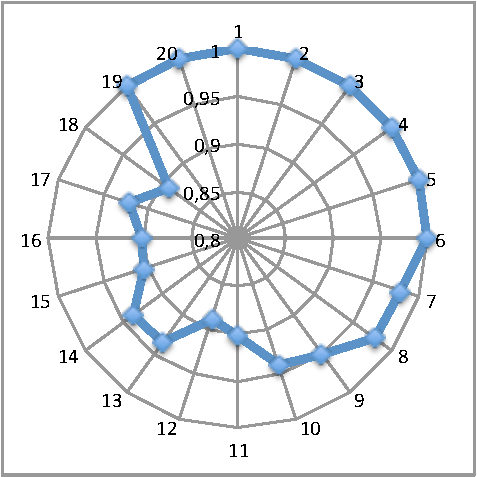
\includegraphics[width=3.9cm]{images/clustering/al-85.pdf}} \\[-0.1in]

% \textbf{80\%}
\subfloat{
\includegraphics[height=3.9cm]{images/clustering/80.pdf}}
   & \subfloat[13 Clusters]{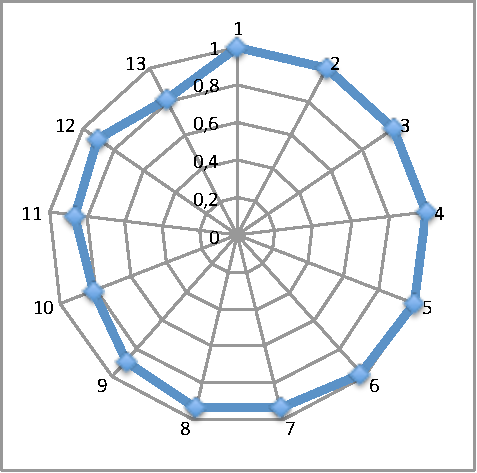
\includegraphics[width=3.9cm]{images/clustering/sl-80.pdf}} 
   & \subfloat[9 Clusters]{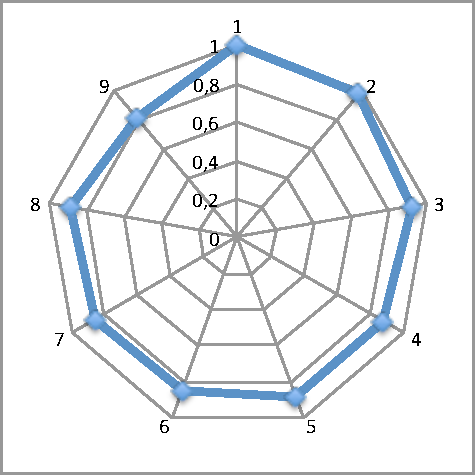
\includegraphics[width=3.9cm]{images/clustering/cl-80.pdf}}
   & \subfloat[7 Clusters]{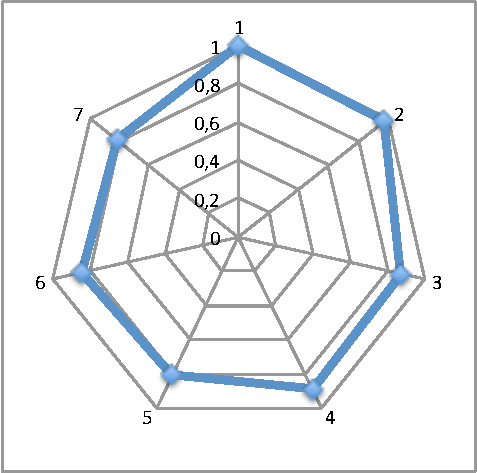
\includegraphics[width=3.9cm]{images/clustering/al-80.pdf}} \\[-0.1in]

% \textbf{75\%}
\subfloat{
\includegraphics[height=3.9cm]{images/clustering/75.pdf}}
   & \subfloat[9 Clusters]{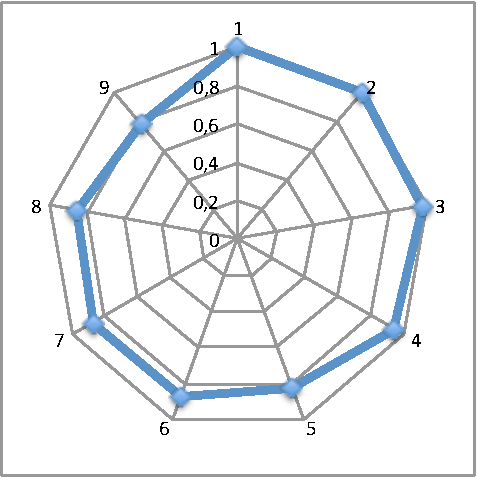
\includegraphics[width=3.9cm]{images/clustering/sl-75.pdf}} 
   & \subfloat[5 Clusters]{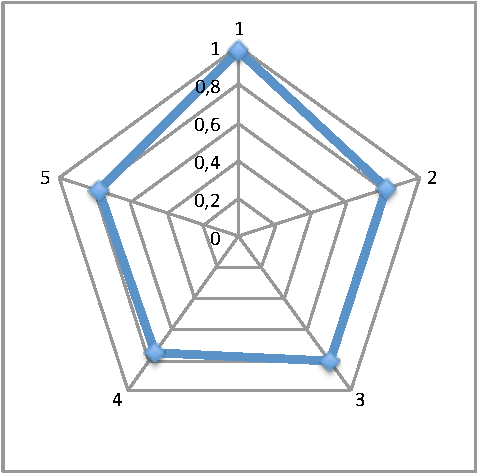
\includegraphics[width=3.9cm]{images/clustering/cl-75.pdf}}
   & \subfloat[5 Clusters]{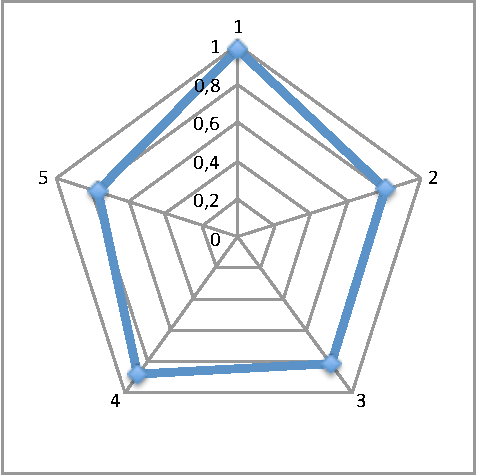
\includegraphics[width=3.9cm]{images/clustering/al-75.pdf}} \\[0in]    
\end{tabular}

\caption{Resultados experimento de Clustering de Tests por Similitud en Cobertura}\figlabel{ap-clustering}
\end{figure}
%================ 

\newpage
\par Luego de una inspección entre los distintos resultados, el parámetro de similitud interna mínima escogido fue de 85\%, ya que los tres resultados generan una cantidad de clusters razonable y con muy buena similitud interna. Entre las tres opciones, se descartó la opción (\emph{Single Link}, 85\%) ya que la mitad de sus clusters son unitarios (condición 3), y tampoco respeta la condición 2, ya que tiene un cluster con más de 30 tests, el siguiente en tamaño 18 (casi la mitad del primero) y el siguiente 10 (casi la mitad del tercero y un tercio del primero) y luego muchos clusters pequeños. 

% Tabla comparativa 3 mejores casos

%== Comparacion entre clusterings
\begin{figure}
\centering
\begin{tabular}{c}
\subfloat[Comparación de los tamaños de cada cluster]{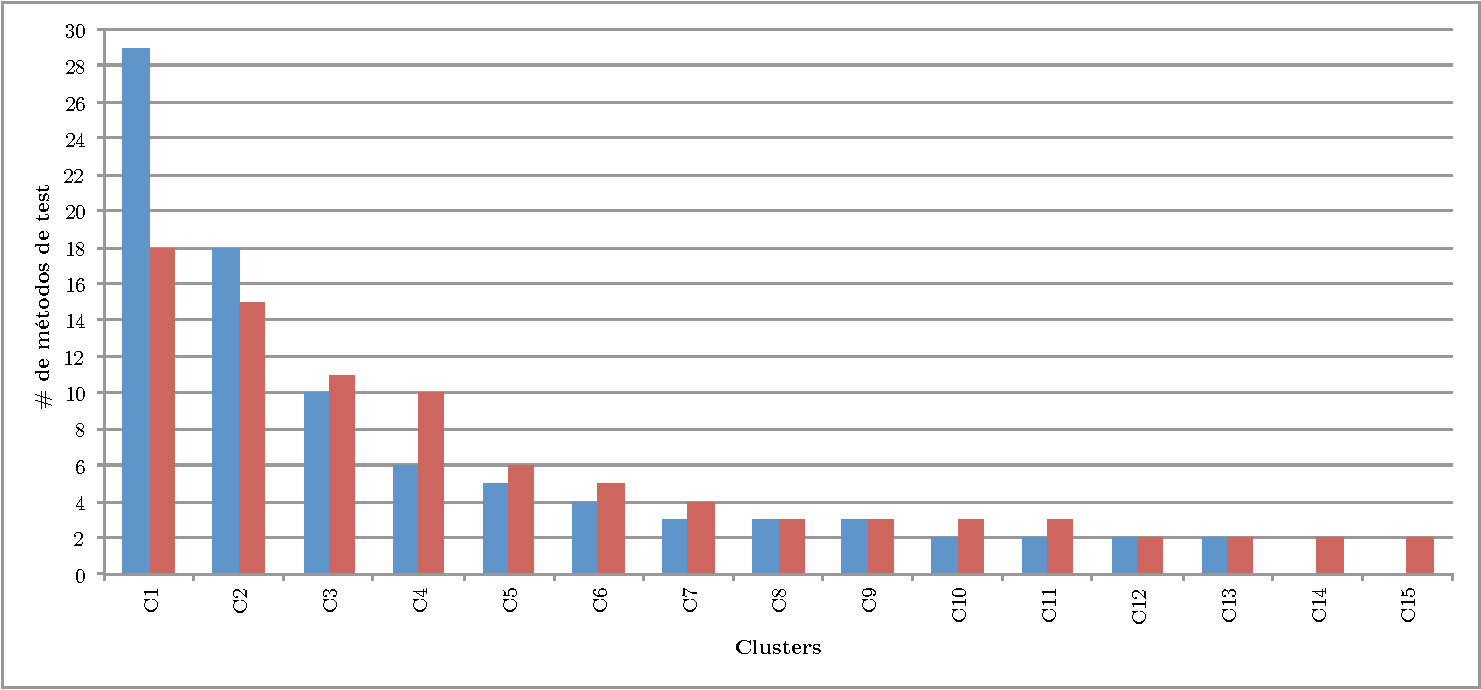
\includegraphics[width=14cm]{images/clustering/comp-tamanos.pdf}} \\[2cm] 
\subfloat[Comparación de la similitud interna de cada cluster]{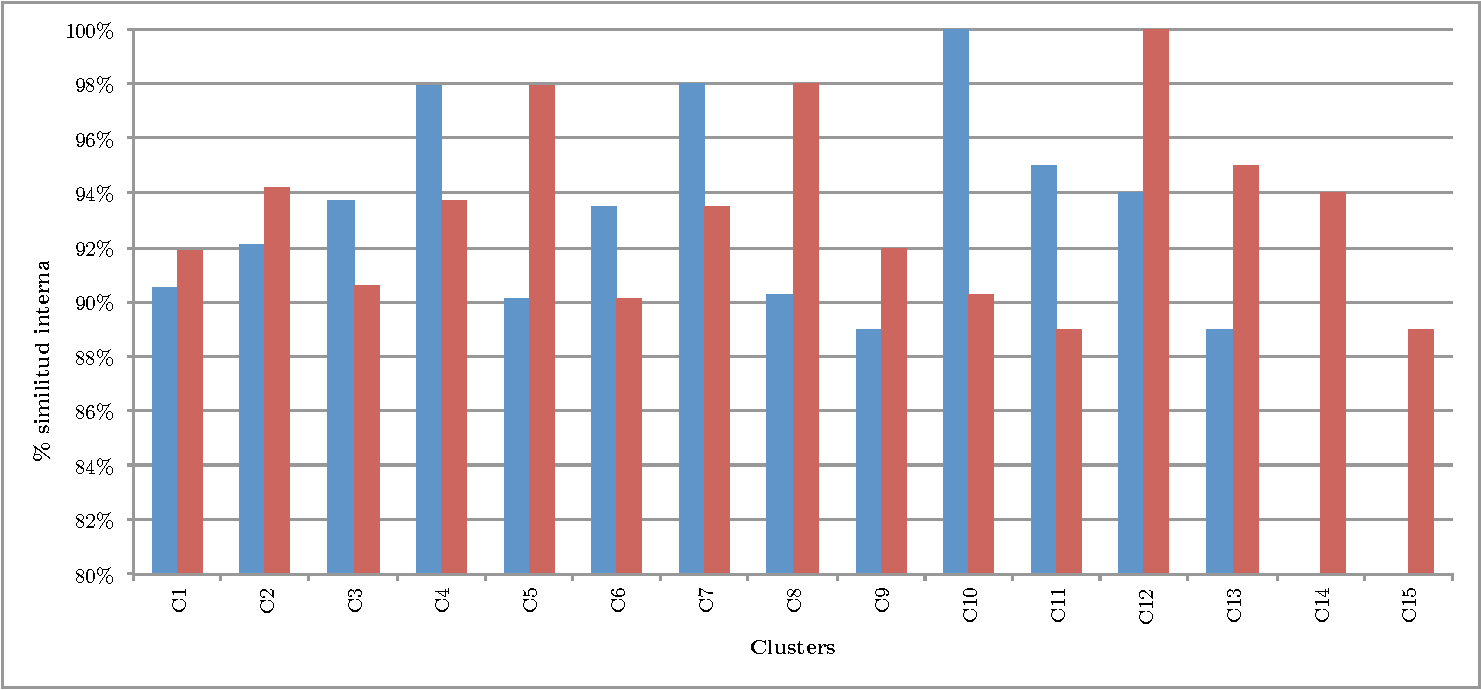
\includegraphics[width=14cm]{images/clustering/comp-sim-int.pdf}}
\end{tabular}
\caption{Análisis comparativo entre los dos mejores agrupamientos}

\footnotesize
\begin{tabular}{rl}
\textbf{Azul}: & \emph{Average Link}, 85\% \\
\textbf{Rojo}: & \emph{Complete Link}, 85\%
\end{tabular}
\figlabel{ap-comp-clus}
\end{figure}


\par Entre las dos alternativas restantes se realizó una comparación mas acuciosa. Por un lado, la alternativa (\emph{Complete Link}, 85\%) genera dos clusters más que (\emph{Average Link}, 85\%) (ver \figref{ap-clustering} (k) y (l)), los dos casos presentan igual número de clusters unitarios. La \figref{ap-comp-clus} muestra los gráficos comparativos según tamaño y similitud interna. En ambos los clusters están ordenados de izquierda a derecha según su tamaño (número de elementos) y en orden decreciente. 

\par La \figref{ap-comp-clus}(a) permite revisar la condición 2. Allí se aprecia que la mejor distribución de los tests se da en (\emph{Complete Link}, 85\%) ya que los clusters no difieren tanto en tamaño. Además en el caso de (\emph{Average Link}, 85\%) se observa un escenario similar al de (\emph{Single Link}, 85\%) con un cluster de gran tamaño, el siguiente la mitad del primero, y así sucesivamente. Inicialmente se pensó en el caso en que el cluster $C_1$ del caso \emph{Average Link} fueran los clusters $C_1$ y $C_2$ de \emph{Complete Link} fusionados, pero luego de una inspección con TestSurgeon determinó que esto no era así y que de hecho los dos clusters $C_1$ y $C_2$ eran bastante distintos ya similitud entre sus elementos en general era menor al 80\% (incluso menor a $s_{min}$). 

\par Esta mejor distribución en el caso de \emph{Complete Link} se explica porque la métrica es más conservadora. Ya que los clusters fusionados en cada paso del algoritmo son los más cercanos considerando los elementos más lejanos de cada cluster. Es decir los tests fusionados son realmente muy cercanos ya que la cota mínima de similitud interna es bastante exigente. En contraparte, \emph{Average Link}, al considerar los promedios de similitudes no toma en cuenta la varianza.

\par La \figref{ap-comp-clus}(b) permite revisar la condición 1. En este caso el contraste es aun mayor ya que en general los clusters de (\emph{Complete Link}, 85\%) son más homogéneos, es decir, sus elementos son más similares. Y el cluster más heterogéneo tiene una similitud interna de $89\%$ y es el único caso. Además el 60\% de los clusters $s >= 92\%$ lo cual habla de clusters equilibrados en tamaño y muy similares entre ellos. Es decir en (\emph{Complete Link}, 85\%) además de reducir el número total de comparaciones, los pares de tests a comparar son entre sí muy similares (en cada cluster).

\par Finalmente, traduciendo lo anterior a número de comparaciones se tiene: (\emph{Average Link}, 85\%) = 648 comparaciones, y (\emph{Complete Link}, 85\%) con \textbf{405 comparaciones}. Por lo cual la configuración escogida es {\bf (\emph{Complete Link}, 85\%)}.

\section{Conclusión}

\par En conclusión se obtuvo una reducción de comparaciones que incialmente eran 4.560 a 405. Luego del agrupamiento se descartó el 91\% de las comparaciones iniciales las cuales eran innecesarias puesto que la cobertura entre los elementos no daba lugar a un caso de interés. Esto significa una inmensa reducción de tiempo innecesario para el desarrollador para enfocarse en los casos realmente interesantes. 




